% 中文版，用 xelatex 编译：latexmk -xelatex estimation_note_zh
\documentclass[11pt,UTF8]{ctexart}
\usepackage[margin=1in]{geometry}
\usepackage{amsmath,amssymb,amsthm,booktabs,graphicx,float,xcolor}
\usepackage[round,authoryear]{natbib}
\usepackage[hidelinks]{hyperref}

\newcommand{\E}{\mathbb{E}}
\newcommand{\ES}{\mathrm{ES}}
\newcommand{\Var}{\operatorname{Var}}
\newcommand{\tr}{\operatorname{tr}}
\newcommand{\vecop}{\operatorname{vec}}
\renewcommand{\arraystretch}{1.12}
\setlength{\abovecaptionskip}{4pt}
\setlength{\belowcaptionskip}{6pt}
\renewcommand{\refname}{参考文献}

\newtheorem{proposition}{命题}
\newtheorem{corollary}{推论}
\newtheorem{lemma}{引理}
\renewcommand{\proofname}{证明}

\title{分布误设下的结构化估计：\\
\large 相对尾部风险估计量的有限样本与渐近性质}
\author{Shangrong Li\thanks{研究笔记，未经同行评审。代码、模拟缓存以及生成全部数字的 notebook：
\url{https://github.com/lshangro-png/tail-risk-cn}，目录 \texttt{studies/09\_estimation\_vs\_decision}。
全部结果来自模拟，均可重新生成。本文译自英文版。}}
\date{2026 年 11 月}

\begin{document}
\maketitle

\begin{abstract}
\noindent
基于预期损失（ES）的组合决策只取决于 ES 对组合的排序，而不取决于 ES 的水平。在椭圆分布下，两个组合的 ES 之比等于它们的标准差之比，
因此即使分布设定错误，也可能无偏地估计相对尾部风险。本文研究这一结论何时成立，以及三种 ES 比值估计量的表现：
样本协方差（``高斯''）插件、Tyler 的无分布形状估计量和历史模拟法（HS）。理论方面，我们给出总体层面的结论及其失效条件
（均值非零时，比值保持协方差形式当且仅当两个组合的夏普比率相同），三种估计量的一致性，以及它们的渐近分布。
椭圆分布下样本协方差比值的渐近方差为 $(1+\kappa)(1-\rho^2)$，Tyler 比值对所有椭圆分布都是 $\frac{d+2}{d}(1-\rho^2)$，
所以当且仅当 Student-$t$ 的自由度满足 $\nu<d+4$ 时 Tyler 更有效。$2<\nu<4$ 时，样本协方差比值以更慢的速度 $T^{-(1-2/\nu)}$
收敛到 $(\nu/2)$-稳定分布。在六个资产、七个共享同一协方差矩阵的分布、每格 5{,}000 次重复的模拟中，每一条预测都得到验证：
高斯插件 3--9\% 的水平偏差在比值中消失，它相对 HS 的优势完全来自方差，Tyler 在 $t_4$ 下把误差减半，
样本协方差比值的四分位距在 $t_3$ 下以斜率 $-0.332$ 收缩（预测为 $-1/3$）。结构只在成立时才有帮助：
在协方差相同的非椭圆崩盘混合分布下，样本协方差比值偏差 9--59\%，Tyler 比值偏差 27--84\%，只有 HS 是一致的。
\end{abstract}

% ---------------------------------------------------------------------------
\section{引言}

用错误的分布估计 ES，水平就会出错。如果收益服从自由度为 4 的 Student-$t$ 分布而风险经理假设正态，她算出的 95\% ES 大约低 9\%。
这是否要紧，取决于估计值用来做什么。最小化 ES 或让各资产的 ES 贡献相等，只需要组合按 ES 的\emph{排序}。
同一仓库中较早的一项模拟研究（09 篇）发现，在六资产宇宙中，设定错误的高斯插件做出的决策比非参数的 HS 估计量更好，
尽管 HS 对 ES 水平估计得更准；能预测决策质量的是两个组合 ES 之\emph{比}的误差，而不是水平的误差。

本文把这一观察变成一个估计问题：\emph{当完整的分布模型错误时，正确设定的那部分结构能否仍然给出准确、稳健、具有良好理论性质的估计量？}
估计目标是相对尾部风险
\[
\theta=\frac{\ES_q(-w_1^\top X)}{\ES_q(-w_2^\top X)} .
\]
椭圆分布下 $\theta$ 只通过离散矩阵的形状依赖于它（第~\ref{sec:pop}~节），由此自然引出三种估计量：样本协方差、只估计形状的估计量（Tyler 的 M 估计量），
以及不利用任何结构的 HS。我们研究它们的一致性、渐近分布和有限样本表现，以及结构失效的条件。

大多数基本结论是已知的。椭圆分布下 ES 的线性表示是教科书内容 \citep{mcneil2015}，Tyler 估计量及其渐近协方差来自 \citet{tyler1987}，
经验 ES 的渐近正态性见 \citet{chen2008}。本文所做的是把它们用于 ES 比值，并推导出几个我们没有见到以这种形式陈述过的推论：
非零均值破坏比值的精确条件（命题~\ref{prop:bound}），比值估计量渐近方差的闭式解与效率交叉点 $\nu<d+4$（推论~\ref{cor:vg}--\ref{cor:eff}），
以及四阶矩不存在时样本协方差比值的收敛速度与稳定极限（命题~\ref{prop:stable}）。第~\ref{sec:contrib}~节逐条列出哪些结论引自文献、
哪些是本文推导、哪些只是模拟证据。我们没有穷尽地检索文献，部分推导结果可能已在别处出现。

% ---------------------------------------------------------------------------
\section{设定}\label{sec:setting}

$X_1,\dots,X_T$ 是 $d$ 个资产独立同分布的日收益，均值为 $\mu$，协方差为 $\Sigma$。组合 $w$ 的损失为 $L_w=-w^\top X$，$\sigma_w^2=w^\top\Sigma w$。
对 $\E|L|<\infty$ 的损失 $L$，$\ES_q(L)=\frac1{1-q}\int_q^1\mathrm{VaR}_u(L)\,du$。我们固定两个组合：带约束的最小方差组合 $w_1$
（不做空，单资产不超过 40\%）与等权组合 $w_2$，记 $\rho=\mathrm{Corr}(L_{w_1},L_{w_2})$，$U_j=(L_{w_j}-\E L_{w_j})/\sigma_{w_j}$。
\emph{水平}的估计目标是 $\ES_q(L_{w_2})$，\emph{形状}的估计目标是 $\theta$。定义 $g(M)=\sqrt{w_1^\top Mw_1/w_2^\top Mw_2}$，
$\theta_G=g(\Sigma)=\sigma_{w_1}/\sigma_{w_2}$。

\paragraph{估计量。}
(i) \emph{高斯插件}：$\widehat{\ES}=k^N_q\sqrt{w^\top S_Tw}$，$S_T$ 为样本协方差，$k^N_q=\phi(\Phi^{-1}(q))/(1-q)$ 为正态常数；
它的比值是 $\hat\theta_G=g(S_T)$，与 $k^N_q$ 无关。(ii) \emph{Tyler 插件}：$\hat\theta_{\mathrm{Ty}}=g(\hat V_T)$，其中 $\hat V_T$ 解
$\hat V=\frac dT\sum_t Y_tY_t^\top/(Y_t^\top\hat V^{-1}Y_t)$，$\tr\hat V=d$，$Y_t=X_t-\bar X$。它只用到方向 $Y_t/\|Y_t\|$。
(iii) \emph{HS}：最差 $\lceil(1-q)T\rceil$ 个损失的平均，$\hat\theta_{HS}$ 为两个这样的平均之比。

\paragraph{数据生成过程。}
六个资产的波动率与相关结构仿照沪深 300、中证 500、标普 500、中国国债、黄金和布伦特原油（$d=6$，$\sigma_{w_1}/\sigma_{w_2}=0.535$，$\rho=0.743$）。
七个 DGP 的均值（零）与协方差完全相同，只有尾部不同：高斯；单位方差的多元 Student-$t_\nu$，$\nu\in\{3,4,5,8,15\}$；
以及非椭圆的\emph{崩盘混合}：每天以 1\% 的概率出现一次随机幅度的联合冲击，风险资产下跌、国债和黄金上涨，之后线性变换回共同的协方差。
样本量 $T\in\{125,250,500,1000,2000,4000\}$ 日，$q\in\{0.95,0.975,0.99\}$，每格 5{,}000 次重复；所有估计量在同一批样本上计算。
椭圆 DGP 的真值有解析式，崩盘混合的真值来自 $10^7$ 天的样本。误差用相对误差 $\hat\theta/\theta-1$ 表示，单位为 \%。

% ---------------------------------------------------------------------------
\section{总体层面的结论}\label{sec:pop}

\begin{proposition}[椭圆分布下的 ES]\label{prop:es}
设 $X\sim E_d(\mu,\Sigma,\psi)$ 非退化且 $\E\|X\|<\infty$。存在只依赖 $(q,\psi)$ 的常数 $k_q>0$，使得对所有 $w$，
$\ES_q(L_w)=-w^\top\mu+k_q\sigma_w$。若 $\mu=0$，则无论生成元 $\psi$ 与水平 $q$ 如何都有 $\theta=\theta_G$，
且把 $\Sigma$ 换成 $c\Sigma$ 时 $\theta$ 不变。
\end{proposition}

这一表示是标准结论 \citep[第~6~章]{mcneil2015}；附录~\ref{app:pop} 给出简短证明，包括 $k_q>0$，它保证比值有定义。
后面的一切都由两个推论驱动。第一，插件 $\hat k\sqrt{w^\top\hat\Sigma w}$ 对任何 $\hat k$ 给出相同的比值：
$t_4$ 下高斯插件在 $q=0.95$ 时有 $k^N_q/k^{t_4}_q-1=-8.9\%$ 的总体水平偏差，这一偏差在比值中抵消。
第二，估计目标是\emph{形状} $\Sigma/\tr\Sigma$ 的泛函，所以根本不必估计 $\Sigma$ 的整体尺度。
$\mu=0$ 时，在任意可行集上最小化 ES 就是最小化方差；又因为 Euler ES 贡献 $w_i\partial_{w_i}\ES$ 的份额与方差贡献的份额相同，
ES 平价就是波动率平价 \citep{tasche1999}。因此水平误差永远不会改变这些决策。

\begin{proposition}[比值何时失效]\label{prop:bound}
(i) 在命题~\ref{prop:es} 的假设下，记 $SR_j=w_j^\top\mu/\sigma_{w_j}$，并设 $SR_2<k_q$，从而 $\ES_q(L_{w_2})>0$。则
$\theta=\theta_G(1-SR_1/k_q)/(1-SR_2/k_q)$，且 $\theta=\theta_G$ 当且仅当 $SR_1=SR_2$。
(ii) 没有椭圆性时，即使均值为零、协方差正确，$\theta=\theta_G$ 也可能不成立。
\end{proposition}

(i) 直接由命题~\ref{prop:es} 得到。均值非零时，生成元通过 $k_q$ 重新进入比值，分布误设又变得重要；
不过在日频上影响很小（相对误差约为 $(SR_2-SR_1)/k_q$，日夏普比率在 0.02 左右时只有千分之几）。
对 (ii)，取相互独立的 $X_1\sim N(0,1)$ 与以各 $\frac12$ 的概率取 $\pm1$ 的 $X_2$：两者方差都为 1，所以 $\theta_G=1$，
但 $\ES_{0.95}(-X_1)/\ES_{0.95}(-X_2)=2.06$。崩盘混合是一个六维的例子：在 $q=0.95,0.975,0.99$ 时其总体比值 $\theta$
分别为 0.49、0.43 和 0.34，而 $\theta_G=0.535$。

% ---------------------------------------------------------------------------
\section{渐近理论}\label{sec:asy}

全部证明见附录~\ref{app:asy}。关键事实是 $g$ 对尺度不变，所以它的梯度
$G=\frac{\theta_G}2(w_1w_1^\top/\sigma_{w_1}^2-w_2w_2^\top/\sigma_{w_2}^2)$ 满足 $\tr(G\Sigma)=0$：任何与 $\Sigma$ 成比例的误差都不进入。

\begin{proposition}[一致性]\label{prop:cons}
(a) 若 $\E\|X\|^2<\infty$，则对任意分布 $\hat\theta_G\to\theta_G$ 几乎必然成立。
(b) 若 $X$ 为绝对连续的椭圆分布、中心已知且 $T>d$，则无需任何矩条件 $\hat\theta_{\mathrm{Ty}}\to\theta_G$ 几乎必然成立 \citep{tyler1987}。
(c) 若 $\E|L_{w_j}|<\infty$，则 $\hat\theta_{HS}\to\theta$ 几乎必然成立 \citep{acerbi2002}。
\end{proposition}

前两个极限对任何分布都是 $\theta_G$，只在椭圆族中才等于 $\theta$。崩盘混合下，在 $2\times10^6$ 天样本上算出的 Tyler 极限为 $0.622$，
比 $\theta_G$ 离 $\theta$ 更远。

\begin{proposition}[样本协方差]\label{prop:clt}
若 $\E\|X\|^4<\infty$，则 $\sqrt T(\hat\theta_G/\theta_G-1)\to N(0,V_G)$，其中 $V_G=\frac14\Var(U_1^2-U_2^2)$。
\end{proposition}

\begin{corollary}\label{cor:vg}
若 $X$ 为椭圆分布，峰度参数 $\kappa=\E U^4/3-1$，则 $V_G=(1+\kappa)(1-\rho^2)$。对单位方差的 $t_\nu$（$\nu>4$），$1+\kappa=(\nu-2)/(\nu-4)$。
\end{corollary}

\begin{proposition}[Tyler]\label{prop:tyler}
若 $X$ 为绝对连续的椭圆分布，则 $\sqrt T(\hat\theta_{\mathrm{Ty}}/\theta-1)\to N(0,V_{\mathrm{Ty}})$，
其中 $V_{\mathrm{Ty}}=\frac{d+2}d(1-\rho^2)$，对所有生成元都相同，不需要矩条件。中心已知时这由 \citet{tyler1987} 推出；
对本文使用的样本均值中心化，我们只给出证明要点。
\end{proposition}

\begin{corollary}\label{cor:eff}
对单位方差的 $t_\nu$（$\nu>4$），$V_{\mathrm{Ty}}/V_G=(d+2)(\nu-4)/\{d(\nu-2)\}$，所以 Tyler 渐近更有效当且仅当 $\nu<d+4$。
正态分布下它的效率为 $d/(d+2)$。
\end{corollary}

\begin{proposition}[HS]\label{prop:hs}
若 $\E L_{w_j}^2<\infty$ 且 $L_{w_j}$ 在其 VaR 处密度为正，则 $\sqrt T(\hat\theta_{HS}/\theta-1)\to N(0,V_{HS})$，
其中 $V_{HS}=\Var(\mathrm{IF}_1/\ES_1-\mathrm{IF}_2/\ES_2)$，$\mathrm{IF}_j=v_j+(L_{w_j}-v_j)_+/(1-q)-\ES_j$ \citep{chen2008}。
\end{proposition}

\begin{proposition}[四阶矩不存在]\label{prop:stable}
设 $X=\mu+\sqrt W Z$，$Z\sim N(0,\Sigma_0)$ 与 $W>0$ 独立，且 $P(W>x)\sim cx^{-\alpha}$。单位方差的 $t_\nu$ 有 $\alpha=\nu/2$。
(a) 若 $1<\alpha<2$，则 $(T/a_T)(\hat\theta_G-\theta)$ 收敛到一个 $\alpha$-稳定分布，$a_T\propto T^{1/\alpha}$；误差为 $T^{-(1-2/\nu)}$ 量级，
极限分布的方差无穷。(b) 若 $\alpha=2$（$\nu=4$），则 $\sqrt{T/\log T}\,(\hat\theta_G-\theta)$ 渐近正态。
\end{proposition}

证明利用了尺度不变性：$\hat\theta_G-\theta$ 由 $\frac1T\sum_tW_t\eta_t$ 驱动，其中 $\eta_t=\tr(G(Z_tZ_t^\top-\Sigma_0))$，
因为 $(W_t-\E W)\Sigma_0$ 这一项正好消失。Breiman 引理使 $W_t\eta_t$ 成为指数为 $\alpha$ 的正则变化变量，广义中心极限定理给出稳定极限。
由于极限方差无穷，收敛速度不能从 $\hat\theta_G$ 方差的衰减中读出；分位数则会收敛，所以四分位距按 $T^{-(1-2/\nu)}$ 收缩。

% ---------------------------------------------------------------------------
\section{模拟证据}\label{sec:sim}

\paragraph{水平与形状。}
表~\ref{tab:decomp} 分解了 $T=1000$、$q=0.95$ 时的误差。高斯插件的水平误差主要是偏差，从 $t_{15}$ 的 $-3\%$ 到 $t_4$ 的 $-9\%$，
等于总体常数 $k^N_q/k_q-1$；$T=4000$ 时，$\nu\ge4$ 的情形下偏差占其水平 MSE 的 85--94\%。同一估计量在比值上，
所有椭圆 DGP 在 $T\ge1000$ 时偏差都不超过 0.5\%，每一格中偏差占 MSE 的比例都低于 1\%。HS 在两者上都几乎无偏，只有 $O(1/T)$ 的小样本偏差。
因此在椭圆族中，高斯插件在比值上的优势完全是方差上的优势：正态分布下，它的渐近方差在 $q=0.95,0.975,0.99$ 时分别只有 HS 的 30\%、21\% 和 12\%。
比值估计量不依赖 $q$，而 HS 的尾部观测随 $q$ 提高而减少。崩盘混合下比值偏差在 $T=1000$ 时为 $+9.9\%$，且不随样本消失（渐近值为 $+8.9\%$）。

\begin{table}[H]
\centering\small
\caption{相对误差的偏差与标准差（\%），$T=1000$，$q=0.95$，5{,}000 次重复。}
\label{tab:decomp}
\begin{tabular}{lrrrrrrrr}
\toprule
 & \multicolumn{4}{c}{水平：$\mathrm{ES}(L_{\mathrm{EW}})$} & \multicolumn{4}{c}{形状：ES 比值 $\theta$} \\
\cmidrule(lr){2-5}\cmidrule(lr){6-9}
 & \multicolumn{2}{c}{高斯插件} & \multicolumn{2}{c}{HS} & \multicolumn{2}{c}{高斯插件} & \multicolumn{2}{c}{HS} \\
\cmidrule(lr){2-3}\cmidrule(lr){4-5}\cmidrule(lr){6-7}\cmidrule(lr){8-9}
DGP & 偏差 & 标准差 & 偏差 & 标准差 & 偏差 & 标准差 & 偏差 & 标准差 \\
\midrule
高斯 & $-$0.07 & 2.25 & $-$0.63 & 3.80 & $+$0.06 & 2.11 & $+$0.13 & 3.81 \\
$t_{15}$ & $-$2.89 & 2.49 & $-$0.87 & 4.48 & $+$0.03 & 2.32 & $+$0.26 & 4.32 \\
$t_8$ & $-$5.33 & 2.82 & $-$0.81 & 5.21 & $+$0.05 & 2.60 & $+$0.13 & 4.76 \\
$t_5$ & $-$7.96 & 3.83 & $-$0.83 & 6.43 & $+$0.03 & 3.34 & $+$0.15 & 5.63 \\
$t_4$ & $-$9.15 & 5.59 & $-$0.97 & 7.56 & $+$0.17 & 4.85 & $+$0.25 & 6.14 \\
$t_3$ & $-$8.51 & 25.15 & $-$0.78 & 11.82 & $+$0.50 & 10.68 & $+$0.31 & 7.82 \\
崩盘混合 & $-$14.31 & 7.86 & $-$0.81 & 12.98 & $+$9.87 & 7.14 & $+$1.14 & 8.24 \\
\bottomrule
\end{tabular}
\end{table}

\paragraph{三种比值估计量。}
表~\ref{tab:three} 与图~\ref{fig:tvar} 加入了 Tyler。在每个椭圆 DGP、每个样本量下，它的 $T\cdot\Var$ 都在 0.57 到 0.64 之间，
理论值 $V_{\mathrm{Ty}}=0.60$，且不随 $\nu$ 变化。样本协方差插件在 $\nu\ge8$ 时与 $V_G$ 吻合，在 $t_5$ 下缓慢逼近；
在 $t_4$ 和 $t_3$ 下它的 $T\cdot\Var$ 随 $T$ 持续上升，分别从 1.4 升到 3.2、从 2.8 升到 13.6。推论~\ref{cor:eff} 的交叉点在 $\nu=10$：
平方误差的配对比较在 $t_3$--$t_8$ 下每个 $T$ 都偏向 Tyler，在 $t_{15}$ 与高斯下每个 $T$ 都偏向样本协方差（$t$ 统计量绝对值在 2.5 到 21 之间）。
$t_4$、$T=1000$ 时，Tyler 的 RMSE 只有样本协方差的一半（2.40\% 对 4.85\%）；$t_3$ 时不到四分之一。在每个椭圆 DGP 中 Tyler 都优于 HS。

\begin{table}[H]
\centering\small
\caption{ES 比值估计量，$q=0.95$。粗体：RMSE 最小。$T\cdot\Var$ 为模拟的相对误差方差乘以 $T$；三列``理论值''为命题~\ref{prop:clt}--\ref{prop:hs}
给出的渐近方差（$\infty$：没有有限的渐近方差；--：没有闭式解）。}
\label{tab:three}
\begin{tabular}{lrrrrrrrrr}
\toprule
 & \multicolumn{3}{c}{RMSE（\%），$T=1000$} & \multicolumn{3}{c}{$T\cdot\mathrm{Var}$，$T=4000$} & \multicolumn{3}{c}{理论值} \\
\cmidrule(lr){2-4}\cmidrule(lr){5-7}\cmidrule(lr){8-10}
DGP & 高斯 & Tyler & HS & 高斯 & Tyler & HS & $V_G$ & $V_{\mathrm{Ty}}$ & $V_{HS}$ \\
\midrule
高斯 & \textbf{2.11} & 2.43 & 3.81 & 0.44 & 0.59 & 1.44 & 0.45 & 0.60 & 1.49 \\
$t_{15}$ & \textbf{2.32} & 2.46 & 4.33 & 0.56 & 0.62 & 1.91 & 0.53 & 0.60 & 1.87 \\
$t_8$ & 2.60 & \textbf{2.44} & 4.77 & 0.67 & 0.60 & 2.34 & 0.67 & 0.60 & 2.32 \\
$t_5$ & 3.34 & \textbf{2.46} & 5.63 & 1.24 & 0.61 & 3.08 & 1.34 & 0.60 & 3.17 \\
$t_4$ & 4.85 & \textbf{2.40} & 6.14 & 3.19 & 0.60 & 4.06 & $\infty$ & 0.60 & 3.96 \\
$t_3$ & 10.69 & \textbf{2.45} & 7.83 & 13.59 & 0.61 & 6.35 & $\infty$ & 0.60 & 6.38 \\
崩盘混合 & 12.18 & 26.72 & \textbf{8.32} & 5.56 & 1.07 & 6.78 & 5.74 & -- & 6.61 \\
\bottomrule
\end{tabular}
\end{table}

\begin{figure}[H]
\centering
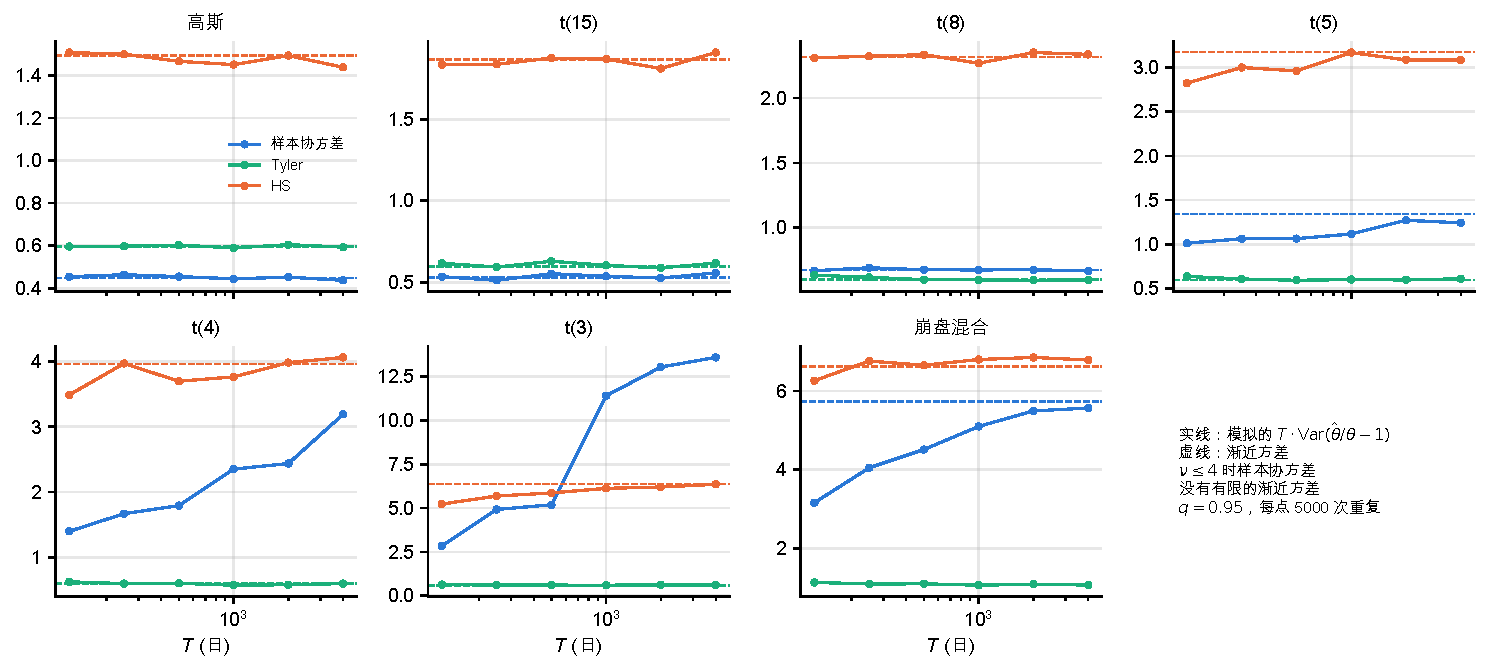
\includegraphics[width=\textwidth]{figures/zh/est_tvar.pdf}
\caption{各样本量下的 $T\cdot\Var(\hat\theta/\theta-1)$，$q=0.95$。虚线：渐近方差。}
\label{fig:tvar}
\end{figure}

\paragraph{收敛速度。}
表~\ref{tab:rates} 把每个估计量误差的对数四分位距对 $\log T$ 回归。$\sqrt T$ 收敛的情形斜率在 $-0.47$ 到 $-0.52$ 之间，
例外是 $t_5$ 下的样本协方差（$-0.459$）和 $t_3$ 下的 HS（$-0.442$），它们在这个 $T$ 范围内收敛较慢。
样本协方差比值的斜率在 $t_3$ 下为 $-0.332$，命题~\ref{prop:stable}(a) 的预测为 $-1/3$；在 $t_4$ 下为 $-0.431$，
$\sqrt{\log T/T}$ 在这个范围内的预测约为 $-0.42$。若改用方差的斜率，则得到 $-0.56$ 和 $-0.75$（$\sqrt T$ 收敛对应 $-1$），
这正是极限方差无穷时应有的现象。

\begin{table}[H]
\centering\small
\caption{$\log\mathrm{IQR}(\hat\theta/\theta-1)$ 对 $\log T$ 的斜率，$T=125,\dots,4000$，$q=0.95$。$\sqrt T$ 收敛对应 $-0.5$。}
\label{tab:rates}
\begin{tabular}{lrrrr}
\toprule
DGP & 预测（样本协方差） & 样本协方差 & Tyler & HS \\
\midrule
高斯 & $-$0.500 & $-$0.504 & $-$0.494 & $-$0.503 \\
$t_{15}$ & $-$0.500 & $-$0.501 & $-$0.499 & $-$0.490 \\
$t_8$ & $-$0.500 & $-$0.505 & $-$0.507 & $-$0.490 \\
$t_5$ & $-$0.500 & $-$0.459 & $-$0.507 & $-$0.473 \\
$t_4$ & $-$0.424 & $-$0.431 & $-$0.514 & $-$0.477 \\
$t_3$ & $-$0.333 & $-$0.332 & $-$0.501 & $-$0.442 \\
\bottomrule
\end{tabular}
\end{table}

\paragraph{置信区间。}
表~\ref{tab:cov} 报告了由命题~\ref{prop:clt}--\ref{prop:hs} 构造的名义 95\% 区间 $\hat\theta(1\pm1.96\sqrt{\hat V/T})$ 的覆盖率，每格 2{,}000 次重复。
Tyler 区间在每个椭圆格子中的覆盖率都在 94.2--95.7\% 之间，宽度不依赖 $\nu$。样本协方差区间在 $\nu\ge8$ 时准确，
在小样本、厚尾时覆盖不足（$t_3$、$T=250$ 时为 89.5\%）。$t_3$ 下它的覆盖率在 $T=4000$ 时回升到 94.1\%，但这没有理论保证：
$\alpha<2$ 时 Student 化统计量的行为类似自归一化和，其极限不是正态分布 \citep{logan1973}；而且区间宽度是 Tyler 的 2.5 倍。
HS 区间从 $T=1000$ 起准确。

\begin{table}[H]
\centering\small
\caption{真实 ES 比值的名义 95\% 区间的覆盖率（\%），$q=0.95$，2{,}000 次重复（蒙特卡洛标准误约 0.5 个百分点），按样本量 $T$ 列出。}
\label{tab:cov}
\begin{tabular}{lrrrrrrrrr}
\toprule
 & \multicolumn{3}{c}{样本协方差} & \multicolumn{3}{c}{Tyler} & \multicolumn{3}{c}{HS} \\
\cmidrule(lr){2-4}\cmidrule(lr){5-7}\cmidrule(lr){8-10}
DGP & 250 & 1000 & 4000 & 250 & 1000 & 4000 & 250 & 1000 & 4000 \\
\midrule
高斯 & 94.4 & 95.5 & 94.5 & 94.8 & 95.2 & 94.8 & 93.2 & 95.2 & 95.0 \\
$t_8$ & 94.0 & 94.0 & 94.5 & 94.5 & 94.8 & 94.2 & 93.2 & 94.5 & 94.8 \\
$t_5$ & 92.5 & 94.0 & 93.5 & 94.5 & 95.5 & 95.1 & 92.6 & 94.3 & 94.2 \\
$t_4$ & 91.9 & 93.9 & 94.5 & 94.6 & 95.7 & 94.2 & 92.7 & 95.0 & 94.7 \\
$t_3$ & 89.5 & 92.8 & 94.1 & 94.2 & 94.5 & 95.0 & 92.2 & 95.1 & 94.2 \\
崩盘混合 & 61.4 & 56.5 & 29.2 & 0.4 & 0.0 & 0.0 & 84.0 & 94.0 & 94.3 \\
\midrule
\multicolumn{10}{l}{\emph{区间宽度中位数（占 $\theta$ 的 \%），$T=4000$}} \\
高斯 & \multicolumn{3}{c}{4.1} & \multicolumn{3}{c}{4.8} & \multicolumn{3}{c}{7.6} \\
$t_4$ & \multicolumn{3}{c}{7.6} & \multicolumn{3}{c}{4.8} & \multicolumn{3}{c}{12.1} \\
$t_3$ & \multicolumn{3}{c}{12.1} & \multicolumn{3}{c}{4.8} & \multicolumn{3}{c}{14.4} \\
崩盘混合 & \multicolumn{3}{c}{12.3} & \multicolumn{3}{c}{4.9} & \multicolumn{3}{c}{15.8} \\
\bottomrule
\end{tabular}
\end{table}

\paragraph{结构失效时。}
崩盘混合下，样本协方差比值与 Tyler 比值收敛到错误的值。记 $\beta=\theta_G/\theta-1$；忽略 $O(1/T)$ 项，
$\mathrm{MSE}_G\approx\beta^2+V_G/T$，$\mathrm{MSE}_{HS}\approx V_{HS}/T$，所以 HS 在 $T^*\approx(V_{HS}-V_G)/\beta^2$ 之后胜出。
用 $10^7$ 天样本上的影响函数算出 $\beta$、$V_G$ 与 $V_{HS}$，$q=0.95,0.975,0.99$ 时 $T^*$ 分别为 110、54 和 6；
模拟中 HS 分别在网格点 250、125 和 125 首次胜出（$q=0.95$ 时 HS 自身的小样本偏差推迟了交叉点）。
图~\ref{fig:crash} 显示，在 $q=0.95$ 和 $0.975$ 时这一近似与模拟的 RMSE 吻合；$q=0.99$ 时，$T=4000$ 下进入 HS 的尾部观测只有约 40 个，
它的小样本偏差使 RMSE 在整个网格上都高于 $\sqrt{V_{HS}/T}$。Tyler 是三者中最差的：它的极限比 $\theta$ 高 27\%、45\% 和 84\%，
样本协方差为 9\%、25\% 和 59\%。Tyler 对大幅观测降权，而这里决定 ES 的恰恰是大幅度的联合崩盘。
基于两种结构化估计量的区间随 $T$ 增大越来越少地覆盖真实比值（Tyler 为 0\%）；只有 HS 区间有效。

\begin{figure}[H]
\centering
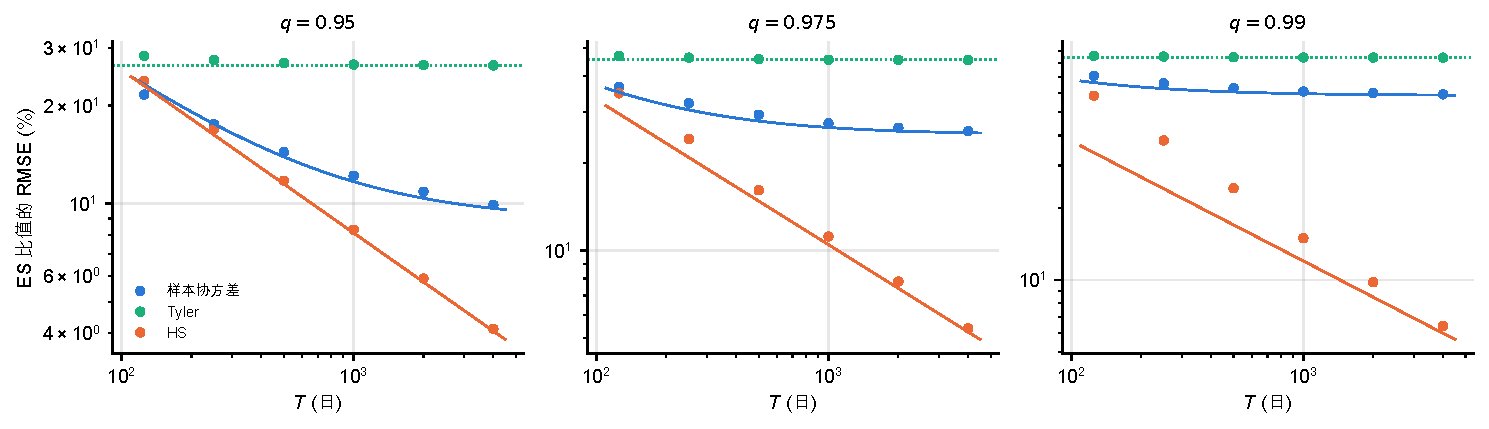
\includegraphics[width=\textwidth]{figures/zh/est_crash.pdf}
\caption{崩盘混合：ES 比值的 RMSE。点：模拟。实线：样本协方差为 $\sqrt{\beta^2+V_G/T}$，HS 为 $\sqrt{V_{HS}/T}$。点线：Tyler 的渐近偏差。}
\label{fig:crash}
\end{figure}

% ---------------------------------------------------------------------------
\section{哪些已知，哪些是本文推导，哪些只是模拟}\label{sec:contrib}

\begin{table}[H]
\centering\small
\begin{tabular}{p{0.50\textwidth}p{0.42\textwidth}}
\toprule
结论 & 来源 \\
\midrule
椭圆分布下 ES $=-w^\top\mu+k_q\sigma_w$；ES 比值 $=\sigma_{w_1}/\sigma_{w_2}$（命题~\ref{prop:es}） & 已知 \citep{mcneil2015}；附有证明 \\
最小 ES $\Leftrightarrow$ 最小方差，ES 平价 $\Leftrightarrow$ 波动率平价 & 已知 \citep{tasche1999,mcneil2015} \\
非零均值：比值保持当且仅当夏普比率相同（命题~\ref{prop:bound}(i)） & 本文推导（初等） \\
三种估计量的一致性（命题~\ref{prop:cons}） & (a) 本文证明；(b)、(c) 引用 \\
$V_G=\frac14\Var(U_1^2-U_2^2)$，椭圆分布下为 $(1+\kappa)(1-\rho^2)$（命题~\ref{prop:clt}、推论~\ref{cor:vg}） & 本文用 Delta 方法推导 \\
$V_{\mathrm{Ty}}=\frac{d+2}d(1-\rho^2)$（命题~\ref{prop:tyler}） & 由 \citet{tyler1987} 加 Delta 方法得到；样本均值中心化只给出要点 \\
效率交叉点 $\nu<d+4$（推论~\ref{cor:eff}） & 本文推导；模拟证实 \\
HS 的渐近正态性（命题~\ref{prop:hs}） & 引用 \citep{chen2008} \\
$2<\nu<4$ 时的速度 $T^{-(1-2/\nu)}$ 与 $(\nu/2)$-稳定极限（命题~\ref{prop:stable}） & 本文用标准工具推导；IQR 斜率证实 \\
误设下的交叉样本量 $T^*$ & 启发式近似；与模拟一致 \\
崩盘混合下 Tyler 劣于样本协方差 & 单个 DGP 的模拟结果 \\
\bottomrule
\end{tabular}
\end{table}

本项目早先的一个非正式版本曾把命题~\ref{prop:stable} 中的极限说成正态的尺度混合。那需要条件 Lindeberg 条件，
而 $W^2$ 的尾指数 $\alpha/2<1$，该条件不成立；正确的极限是稳定分布，收敛速度不受影响。

% ---------------------------------------------------------------------------
\section{局限}

\begin{itemize}
\item \emph{独立性。} 全部理论与模拟都假设收益独立同分布。波动率聚集会同时改变渐近方差和区间的有效性；
09 篇中的动态实验（GJR-GARCH）不在本文理论覆盖范围内。
\item \emph{一个资产宇宙、一对组合。} 结论针对 $d=6$ 的一个协方差矩阵和一对组合。常数 $\rho$ 出现在每个渐近方差中；交叉点 $\nu<d+4$ 随 $d$ 移动。
\item \emph{只有一种非椭圆备择。} 崩盘混合是单一的、刻意设定得很强的偏离。在其他偏离下，误设时样本协方差与 Tyler 的排序可能不同。
\item \emph{证明中的缺口。} 带估计中心的 Tyler 渐近性质（命题~\ref{prop:tyler}）只给出要点，所需的一致性条件没有验证，尽管模拟的方差与公式吻合。
我们没有刻画在单个水平 $q$ 下比值恒等式成立的分布类。
\item \emph{厚尾下的区间。} $2<\nu<4$ 时样本协方差区间没有渐近保证，我们只报告其模拟覆盖率。
\item \emph{与决策的关系。} 比值误差与决策质量之间的联系是 09 篇的模拟证据，不是定理；决策后悔对估计误差的一阶展开留待后续工作。
\end{itemize}

% ---------------------------------------------------------------------------
\section{结论}

当决策取决于相对尾部风险时，只要所依赖的那部分结构正确，设定错误的模型也能无偏地估计它。在椭圆族中，问题于是变成在形状估计量之间选择，
而选择由尾部厚度决定：轻尾时样本协方差最好，$\nu<d+4$ 时 Tyler 估计量更好；四阶矩不存在时样本协方差失去 $\sqrt T$ 速度，Tyler 则保持。
同样的推理也提醒我们不要依赖并不存在的结构：在协方差正确的非椭圆崩盘混合下，形状估计量越稳健，离 ES 比值越远，只有非参数估计量是一致的。
自然的下一步是在选择估计量之前先检验椭圆结构本身，并把渐近理论推广到相依数据。

% ---------------------------------------------------------------------------
\appendix
\section{第~\ref{sec:pop}~节的证明}\label{app:pop}

\begin{proof}[命题~\ref{prop:es} 的证明]
$X-\mu$ 的特征函数为 $\psi(t^\top\Sigma t)$，所以 $w^\top(X-\mu)$ 的特征函数为 $\psi(s^2\sigma_w^2)$。取 $\sigma_{w_0}=1$ 的 $w_0$，令 $Z=w_0^\top(X-\mu)$；
它的特征函数 $\psi(s^2)$ 是实的偶函数，所以 $Z$ 对称，且对每个 $w$ 有 $-w^\top(X-\mu)\overset d=\sigma_wZ$。ES 具有法则不变性、平移等变性和正齐次性，所以
$\ES_q(L_w)=-w^\top\mu+\sigma_w\ES_q(Z)$。令 $f(u)=\mathrm{VaR}_u(Z)$，它单调不减且 $\int_0^1f=\E Z=0$。$f$ 在 $(0,q)$ 和 $(q,1)$ 上的平均值夹住
$f(q^-)\le f(q^+)$，且加权平均为零，所以 $k_q=\ES_q(Z)\ge0$，等号只在 $f$ 几乎处处为常数即 $Z\equiv0$ 时成立，这被非退化性排除。比值的结论随之得到。
\end{proof}

\begin{proof}[命题~\ref{prop:bound} 的证明]
(i) 由命题~\ref{prop:es}，$\theta=(k_q\sigma_{w_1}-w_1^\top\mu)/(k_q\sigma_{w_2}-w_2^\top\mu)$；提出 $k_q\sigma_{w_j}$ 即可。
与 $\theta_G$ 相等当且仅当 $1-SR_1/k_q=1-SR_2/k_q$。(ii) 即正文中的反例：$\ES_{0.95}(-X_1)=k^N_{0.95}=2.063$，$\ES_{0.95}(-X_2)=1$。
\end{proof}

\section{第~\ref{sec:asy}~节的证明}\label{app:asy}

\begin{lemma}\label{lem:g}
对 $c>0$ 有 $g(cM)=g(M)$，且 $Dg(M)[H]=\tr(G_MH)$，其中
\[
G_M=\frac{g(M)}2\left(\frac{w_1w_1^\top}{w_1^\top Mw_1}-\frac{w_2w_2^\top}{w_2^\top Mw_2}\right).
\]
此外 $\tr(G_MM)=0$，并且对 $G=G_\Sigma$ 有 $\tr(G\Sigma G\Sigma)=\frac12\theta_G^2(1-\rho^2)$。
\end{lemma}

\begin{proof}
对 $\log g=\frac12\log(w_1^\top Mw_1)-\frac12\log(w_2^\top Mw_2)$ 求导。对最后一个恒等式，记 $A=w_1w_1^\top$，$B=w_2w_2^\top$：
$\tr(A\Sigma A\Sigma)=\sigma_{w_1}^4$，$\tr(B\Sigma B\Sigma)=\sigma_{w_2}^4$，$\tr(A\Sigma B\Sigma)=\rho^2\sigma_{w_1}^2\sigma_{w_2}^2$。
\end{proof}

\begin{proof}[命题~\ref{prop:cons} 的证明]
(a) 由强大数定律，$S_T=\frac T{T-1}(\frac1T\sum_tX_tX_t^\top-\bar X\bar X^\top)\to\Sigma$ a.s.，且 $g$ 在 $\Sigma$ 处连续。
(b) \citet{tyler1987} 证明了 $\hat V_T\to c\Sigma$ a.s.；再用尺度不变性。(c) 两个经验 ES 都几乎必然收敛 \citep{acerbi2002}，且分母的极限为正。
\end{proof}

\begin{proof}[命题~\ref{prop:clt} 与推论~\ref{cor:vg} 的证明]
记 $Y=X-\mu$，由于 $\sqrt T\,\bar Y\bar Y^\top=o_p(1)$，$\sqrt T(S_T-\Sigma)=T^{-1/2}\sum_t(Y_tY_t^\top-\Sigma)+o_p(1)$。
多元中心极限定理给出 $\sqrt T\vecop(S_T-\Sigma)\to N(0,\Gamma)$，$\Gamma=\mathrm{Cov}(\vecop YY^\top)$。由 Delta 方法与引理~\ref{lem:g}，
$\sqrt T(\hat\theta_G-\theta_G)$ 的渐近方差为 $\Var(\tr(GYY^\top))=\Var(\frac{\theta_G}2(U_1^2-U_2^2))$。椭圆分布下
$\E[Y_iY_jY_kY_l]=(1+\kappa)(\sigma_{ij}\sigma_{kl}+\sigma_{ik}\sigma_{jl}+\sigma_{il}\sigma_{jk})$ \citep{muirhead1982}，
所以 $\E U_j^4=3(1+\kappa)$，$\E U_1^2U_2^2=(1+\kappa)(1+2\rho^2)$，$\Var(U_1^2-U_2^2)=4(1+\kappa)(1-\rho^2)$。
对单位方差的 $t_\nu$，$\E U^4=3(\nu-2)/(\nu-4)$。
\end{proof}

\begin{proof}[命题~\ref{prop:tyler}（中心已知）与推论~\ref{cor:eff} 的证明]
\citet{tyler1987} 证明了
\[
\sqrt T\vecop(\hat V_T-c\Sigma)\to N\Big(0,\ \tfrac{d+2}d(I+K)(c\Sigma\otimes c\Sigma)+\sigma_2\vecop\Sigma\vecop\Sigma^\top\Big),
\]
其中 $K$ 为交换矩阵，系数 $\frac{d+2}d$ 与生成元无关，$\sigma_2$ 只依赖归一化方式。第二项被 $\tr(G\Sigma)=0$ 消去；
第一项给出 $\frac{d+2}d\cdot2\tr(G\Sigma G\Sigma)=\frac{d+2}d\theta^2(1-\rho^2)$。推论：把 $(d+2)(\nu-4)<d(\nu-2)$ 展开，它等价于 $\nu<d+4$。
\end{proof}

\paragraph{估计中心时的证明要点。}
$\hat V_T$ 解 $\frac1T\sum_t\psi(X_t-m,V)=0$，其中
\[
\psi(y,V)=\frac{d\,yy^\top}{y^\top V^{-1}y}-V .
\]
依赖 $y$ 的部分是零次齐次的偶函数，所以它对 $y$ 的导数是 $-1$ 次齐次的奇函数；在 $\E\|Y\|^{-1}<\infty$（$d\ge2$ 时成立）的对称分布下，
其期望为零，因此 $\sqrt T$ 相合的中心估计没有一阶影响。完整证明需要关于 $m$ 的随机等度连续性，本文没有验证。
模拟的 $T\cdot\Var$ 与 $V_{\mathrm{Ty}}$ 一致（表~\ref{tab:three}）。

\begin{proof}[命题~\ref{prop:stable} 的证明]
由尺度不变性，$\hat\theta_G=g(M_T-\bar Y\bar Y^\top)$，$M_T=\frac1T\sum_tW_tZ_tZ_t^\top$，且 $\bar Y\bar Y^\top=O_p(T^{-1})$。
记 $M_T-\Sigma=\frac1T\sum_t[W_tD_t+(W_t-\E W)\Sigma_0]$，$D_t=Z_tZ_t^\top-\Sigma_0$，$\Sigma=\E W\,\Sigma_0$。线性化并利用 $\tr(G\Sigma_0)=0$，
\[
\hat\theta_G-\theta=\frac1T\sum_tW_t\eta_t+O_p(\|M_T-\Sigma\|^2)+O_p(T^{-1}),\qquad\eta_t=\tr(GD_t),
\]
其中 $\eta_t$ 与 $W_t$ 独立，均值为零，各阶矩有限，且 $|\rho|<1$ 时不退化。由 Breiman 引理，$P(W\eta>x)\sim\E[\eta_+^\alpha]P(W>x)$，
$P(W\eta<-x)\sim\E[\eta_-^\alpha]P(W>x)$，所以 $W_t\eta_t$ 两侧尾部都是指数 $\alpha$ 的正则变化。(a) $1<\alpha<2$ 时，
广义中心极限定理 \citep[第~XVII~章]{feller1971} 给出 $a_T^{-1}\sum_tW_t\eta_t\to\mathcal S_\alpha$，$a_T\propto T^{1/\alpha}$，偏斜参数为
$(\E\eta_+^\alpha-\E\eta_-^\alpha)/(\E\eta_+^\alpha+\E\eta_-^\alpha)$。对每个元素同样论证可得 $\|M_T-\Sigma\|=O_p(a_T/T)$，所以余项为 $o_p(a_T/T)$。
(b) $\alpha=2$ 时，$W\eta$ 的截断二阶矩按 $\log x$ 增长，所以 $W\eta$ 属于正态分布的吸引域，$a_T\asymp\sqrt{T\log T}$。
\end{proof}

% ---------------------------------------------------------------------------
\bibliographystyle{plainnat}
\begin{thebibliography}{99}

\bibitem[Acerbi and Tasche(2002)]{acerbi2002}
Acerbi, C. and Tasche, D. (2002). On the coherence of expected shortfall. \emph{Journal of Banking \& Finance},
26(7), 1487--1503.

\bibitem[Chen(2008)]{chen2008}
Chen, S. X. (2008). Nonparametric estimation of expected shortfall. \emph{Journal of Financial Econometrics},
6(1), 87--107.

\bibitem[Feller(1971)]{feller1971}
Feller, W. (1971). \emph{An Introduction to Probability Theory and Its Applications}, Vol.~II, 2nd ed. Wiley.

\bibitem[Logan et~al.(1973)]{logan1973}
Logan, B. F., Mallows, C. L., Rice, S. O. and Shepp, L. A. (1973). Limit distributions of self-normalized sums.
\emph{Annals of Probability}, 1(5), 788--809.

\bibitem[McNeil et~al.(2015)]{mcneil2015}
McNeil, A. J., Frey, R. and Embrechts, P. (2015). \emph{Quantitative Risk Management: Concepts, Techniques and
Tools}, revised ed. Princeton University Press.

\bibitem[Muirhead(1982)]{muirhead1982}
Muirhead, R. J. (1982). \emph{Aspects of Multivariate Statistical Theory}. Wiley.

\bibitem[Tasche(1999)]{tasche1999}
Tasche, D. (1999). Risk contributions and performance measurement. Working paper, Technische Universit\"at
M\"unchen.

\bibitem[Tyler(1987)]{tyler1987}
Tyler, D. E. (1987). A distribution-free M-estimator of multivariate scatter. \emph{Annals of Statistics},
15(1), 234--251.

\end{thebibliography}

\end{document}
